%%
%% This is file `sample-authordraft.tex',
%% generated with the docstrip utility.
%%
%% The original source files were:
%%
%% samples.dtx  (with options: `authordraft')
%% 
%% IMPORTANT NOTICE:
%% 
%% For the copyright see the source file.
%% 
%% Any modified versions of this file must be renamed
%% with new filenames distinct from sample-authordraft.tex.
%% 
%% For distribution of the original source see the terms
%% for copying and modification in the file samples.dtx.
%% 
%% This generated file may be distributed as long as the
%% original source files, as listed above, are part of the
%% same distribution. (The sources need not necessarily be
%% in the same archive or directory.)
%%
%% The first command in your LaTeX source must be the \documentclass command.
%\documentclass[sigconf,authordraft]{acmart}


%%%% As of March 2017, [siggraph] is no longer used. Please use sigconf (above) for SIGGRAPH conferences.

%%%% As of May 2020, [sigchi] and [sigchi-a] are no longer used. Please use sigconf (above) for SIGCHI conferences.

%%%% Proceedings format for SIGPLAN conferences 
%\documentclass[sigplan, anonymous, authordraft]{acmart}

%%%% Proceedings format for conferences using one-column small layout
%\documentclass[acmsmall,authordraft]{acmart}

% NOTE that a single column version is required for submission and peer review. This can be done by changing the \doucmentclass[...]{acmart} in this template to 
\documentclass[manuscript,screen]{acmart}

%%
%% \BibTeX command to typeset BibTeX logo in the docs
\AtBeginDocument{%
  \providecommand\BibTeX{{%
    \normalfont B\kern-0.5em{\scshape i\kern-0.25em b}\kern-0.8em\TeX}}}

%% Rights management information.  This information is sent to you
%% when you complete the rights form.  These commands have SAMPLE
%% values in them; it is your responsibility as an author to replace
%% the commands and values with those provided to you when you
%% complete the rights form.
\setcopyright{acmcopyright}
\copyrightyear{2021}
\acmYear{2021}
\acmDOI{10.1145/1122445.1122456}

%% These commands are for a PROCEEDINGS abstract or paper.
\acmConference[Yokohama '21]{Yokohama '21: ACM CHI Conference on Human Factors in Computing Systems}{May 08--13, 2021}{Yokohama, Japan}
\acmBooktitle{Yokohama '21: ACM CHI Conference on Human Factors in Computing Systems,
  May 08--13, 2021, Yokohama, Japan}
\acmPrice{15.00}
\acmISBN{978-1-4503-XXXX-X/18/06}

%%%%%%%%%%  REMCO'S MACROS  %%%%%%%%%%%%%%%%
\usepackage[normalem]{ulem}
%\usepackage[prologue,dvipsnames,table,xcdraw]{xcolor}
\usepackage{xcolor}
\definecolor{mred}{rgb}{.80,.12,.30}
\definecolor{MRED}{rgb}{.80,.12,.30}
\definecolor{grey}{rgb}{0.5,0.5,0.5}
\definecolor{purple}{rgb}{.75,0,.85}
\definecolor{pistachio}{rgb}{0.58, 0.77, 0.45}

\definecolor{bar-blue}{HTML}{80b1d3}

\definecolor{bar-noXai}{HTML}{8dd3c7}
\definecolor{bar-Qual}{HTML}{ffffb3}
\definecolor{bar-Markup}{HTML}{bebada}
\definecolor{bar-MarkupQ}{HTML}{fb8072}
\definecolor{bar-PredictQ}{HTML}{fdb462}

\newif\ifnotes
\notestrue

\newcommand{\remco}[1]{\ifnotes{\textcolor{mred}{(Remco: #1)}}\fi}
\newcommand{\ab}[1]{\ifnotes{\leavevmode\color{pistachio}{(Ab: #1)}}\else{#1}\fi}
\newcommand{\andrea}[1]{\ifnotes{\textcolor{blue}{(Andrea: #1)}}\else{#1}\fi}
\newcommand{\nina}[1]{\ifnotes{\textcolor{orange}{(Nina: #1)}}\fi}

\let\origcite\cite
\renewcommand{\cite}[1]{\ifnotes\mbox{\origcite{#1}}\else \origcite{#1}\fi}
\newcommand{\strike}[1]{\ifnotes{\color{mred}{\texorpdfstring{\sout{#1}}{#1}}}\fi}
\newcommand{\strikeg}[1]{\ifnotes{\color{grey}{\texorpdfstring{\sout{#1}}{#1}}}\fi}
\newcommand{\add}[1]{\ifnotes{\leavevmode\color{mred}{#1}}\else{#1}\fi}
\newcommand{\replace}[2]{\ifnotes{\strikeg{#1}\add{#2}}\else{#2}\fi}

\newcommand{\cbox}[1]{\raisebox{\depth}{\fcolorbox{black}{#1}{\null}}}

%%%%%%%%%%  END REMCO'S MACROS  %%%%%%%%%%%%%%%%

%%PACKAGES
\usepackage{comment}
\usepackage{float}
\usepackage{arydshln}
\usepackage{threeparttable}
\usepackage{enumitem}
\usepackage{hang}
\usepackage{multirow}
\setlist{nosep}
\usepackage{subcaption}
\usepackage{bchart}
\usepackage[skip=5pt]{caption}
\graphicspath{ {./images/} }



%%
%% Submission ID.
%% Use this when submitting an article to a sponsored event. You'll
%% receive a unique submission ID from the organizers
%% of the event, and this ID should be used as the parameter to this command.
\acmSubmissionID{123-A56-BU3}

%%
%% The majority of ACM publications use numbered citations and
%% references.  The command \citestyle{authoryear} switches to the
%% "author year" style.
%%
%% If you are preparing content for an event
%% sponsored by ACM SIGGRAPH, you must use the "author year" style of
%% citations and references.
%% Uncommenting
%% the next command will enable that style.
%%\citestyle{acmauthoryear}

%%
%% end of the preamble, start of the body of the document source.
\begin{document}

%%
%% The "title" command has an optional parameter,
%% allowing the author to define a "short title" to be used in page headers.
\title[Explainable AI for Machine Translation]{Explainable AI for Machine Translation: Applying principles of Explainable AI to Machine Translation}

%%
%% The "author" command and its associated commands are used to define
%% the authors and their affiliations.
%% Of note is the shared affiliation of the first two authors, and the
%% "authornote" and "authornotemark" commands
%% used to denote shared contribution to the research.
\author{Ab Mosca}
\authornote{Both authors contributed equally to this research.}
\email{amosca01@cs.tufts.edu}\affiliation{%
  \institution{Tufts University}
}

\author{Andrea Brennen}
\authornotemark[1]
\email{abrennen@iqt.org}
\affiliation{%
  \institution{In-Q-Tel Labs}
}

\author{Nina Lopatina}
\email{nlopatina@iqt.org}
\affiliation{%
  \institution{In-Q-Tel Labs}
}
\author{Remco Chang}
\affiliation{\institution{Tufts University}}
\email{remco@cs.tufts.edu}

%%
%% By default, the full list of authors will be used in the page
%% headers. Often, this list is too long, and will overlap
%% other information printed in the page headers. This command allows
%% the author to define a more concise list
%% of authors' names for this purpose.
\renewcommand{\shortauthors}{Mosca and Brennen, et al.}

%%
%% The abstract is a short summary of the work to be presented in the
%% article.
\begin{abstract}
  \section{Abstract}

%Explainable AI (XAI) tools and research efforts seek to provide insight about “black box” AI/ML systems. Many of these efforts, however, overlook the UI/UX (user interface / user experience) aspects of this challenge. Extracting the right information from and about models is crucial, but it is only part of the challenge of explainability; this information must also be presented to someone through an effective interface.

In this paper, we describe the design, development, and evaluation of VeriCAT, a system that visualizes output of a machine translation (MT) quality estimation (QE) model. In 2017, an incorrect machine translation of a Facebook post led to the erroneous arrest of the author. We design VeriCAT with the intent of preventing situations such as this. VeriCAT, short for verification of computer-assisted translation, displays the likely inaccuracy of a machine translation. This enables users to determine whether to trust a specific machine-translated sentence. VeriCAT predicts the sentence-level quality of translations from Russian into English by the FairSeq MT model. Its user interface shows this predicted quality as a quality score for each translated sentence. We evaluate VeriCAT with a quantitative user study to measure how the tool impacts participants’ ability to identify poor quality machine translations. Our evaluation shows the tool significantly increases participants' accuracy in identifying poor quality machine translations. Moreover, we find participants perform their task as accurately with VeriCAT QE scores as with ground truth quality scores. Finally, we provide lessons learned from this study to inform future work.  

%suggest ways in which future work can leverage our UI evaluation to iterate on VeriCAT as an XAI system system. 

\end{abstract}

%%
%% The code below is generated by the tool at http://dl.acm.org/ccs.cfm.
%% Please copy and paste the code instead of the example below.
%%
\begin{CCSXML}
<ccs2012>
<concept>
<concept_id>10003120.10003121.10003122.10010854</concept_id>
<concept_desc>Human-centered computing~Usability testing</concept_desc>
<concept_significance>500</concept_significance>
</concept>
<concept>
<concept_id>10003120.10003145.10003147</concept_id>
<concept_desc>Human-centered computing~Visualization application domains</concept_desc>
<concept_significance>500</concept_significance>
</concept>
</ccs2012>
\end{CCSXML}

\ccsdesc[500]{Human-centered computing~Usability testing}
\ccsdesc[500]{Human-centered computing~Visualization application domains}
%%
%% Keywords. The author(s) should pick words that accurately describe
%% the work being presented. Separate the keywords with commas.
\keywords{User-centered design, Machine Translation Quality Estimation}

%% A "teaser" image appears between the author and affiliation
%% information and the body of the document, and typically spans the
%% page.

%\begin{teaserfigure}
%  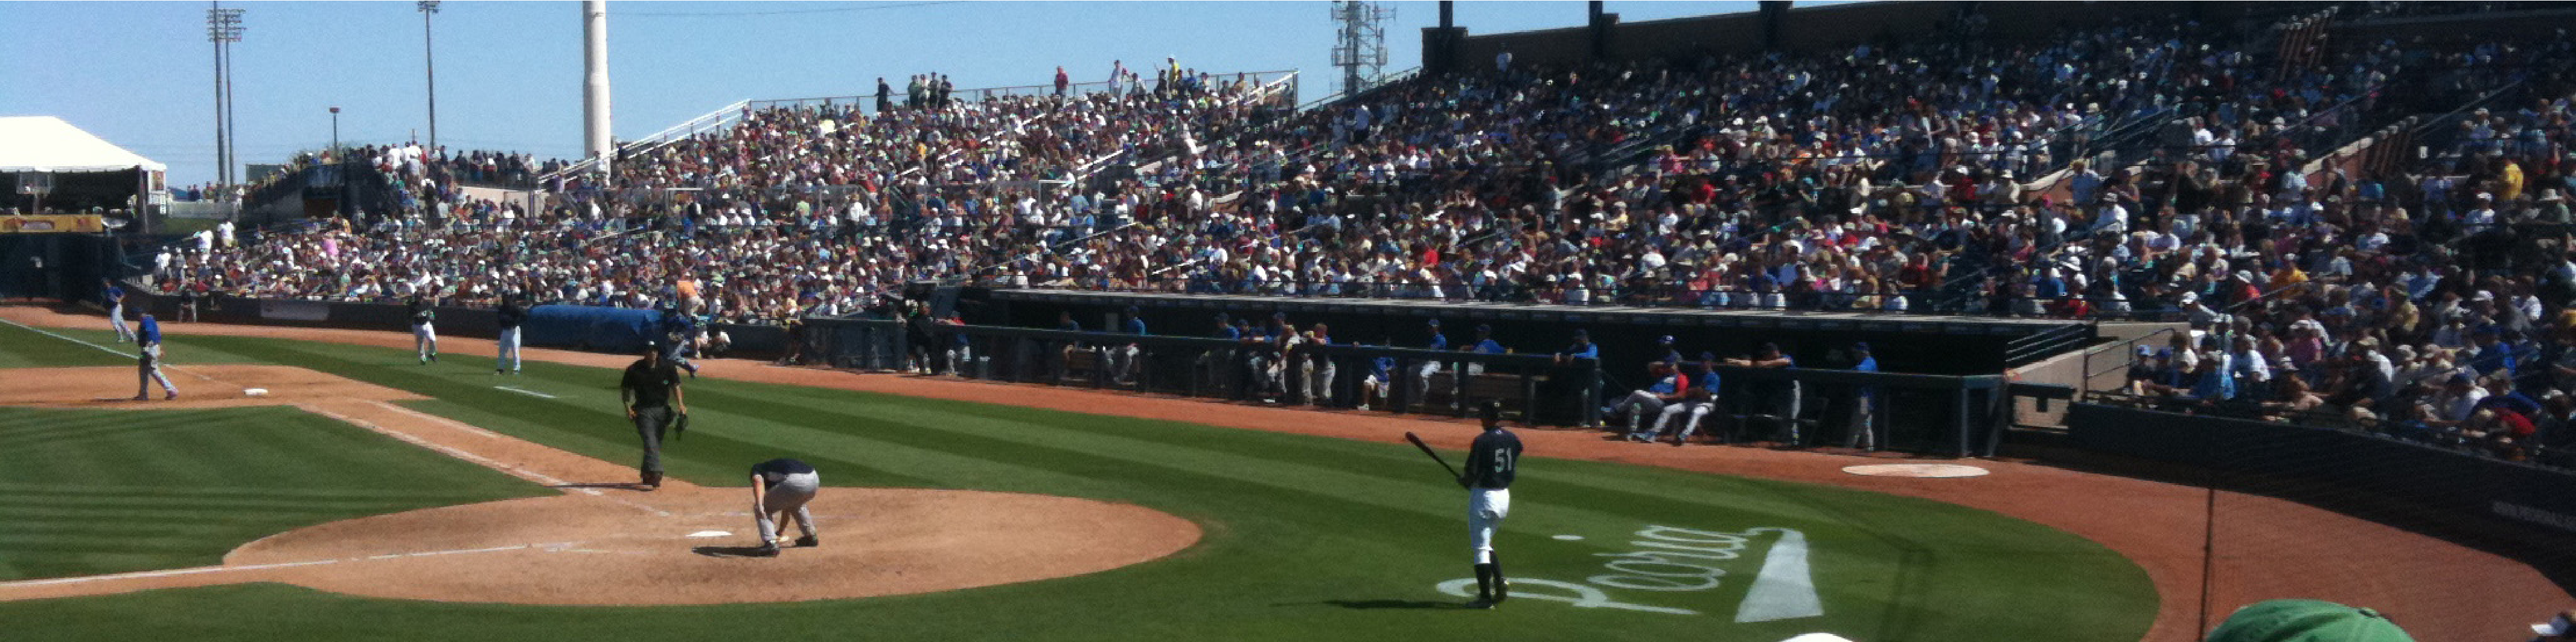
\includegraphics[width=\textwidth]{sampleteaser.pdf}
%  \caption{Seattle Mariners at Spring Training, 2010.}
%  \Description{Enjoying the baseball game from the third-base
 % seats. Ichiro Suzuki preparing to bat.}
%  \label{fig:teaser}
%\end{teaserfigure}

%%
%% This command processes the author and affiliation and title
%% information and builds the first part of the formatted document.
\maketitle

\section{Introduction}

In 2017 Facebook's machine translation (MT) algorithm incorrectly translated a construction worker's Arabic-language post. The original post said ``good morning" in Arabic, but was erroneously translated into Hebrew as ``attack them", leading to the worker's arrest and several hours of questioning. Notably, no Arabic-speakers were asked to verify the machine translation of the post leading up to the arrest~\cite{hernFacebook2017}. For many users of machine translation, it is easy to forget that translated output is susceptible to error and, as illustrated by this situation, some translation errors can lead to severe consequences.
%Analysts might use machine translation in situations where human translators are in short supply. To avoid potentially negative consequences of erroneous translations, analysts would benefit from tools that help them  
%asses the quality of specific passages of translated text.  
Our goal in this work is to develop and evaluate a tool to help users determine when, and whether, to trust machine translation. 

To that end, we present and evaluate VeriCAT, which stands for Verification of Computer-Assisted Translation. VeriCAT is designed to help those using machine translation assess the quality of translated text. In particular, we focus on text snippets that have been translated from Russian into English by the FairSeq model ~\cite{ott-etal-2019-fairseq}. 
VeriCAT consists of a Quality Estimation (QE) model combined with an easy-to-use interface. The objective of QE is to train a machine learning model to predict a quality score for translated text that is similar to what a human would assign to that translation~\cite{mauvcec2019machine}. VeriCAT's QE model is a trained version of OpenKiwi’s predictor-estimator model \cite{Kim2017PredictorEstimatorUM}. VeriCAT's interface shows users the output of the QE model -- a predicted quality score (some value out of a possible 100) for individual sentences of machine-translated text (Figure \ref{fig:p3_predicted_quality}).

VeriCAT is novel in using the output of a Quality Estimation model to provide context to MT users. Typically, QE is used by developers of MT models for validation and model improvement. However, we believe predicted quality scores can also benefit users of translated text, by helping them determine when and whether to trust a particular machine translated sentence. While many MT accuracy metrics (such as BLEU score \cite{papineni-etal-2002-bleu}) provide information about the accuracy of a MT model in general, QE serves as a metric for \textit{individual sentences}. 
 
We evaluate VeriCAT with a quantitative user study, where users are asked to perform an analogous task to that which motivates the development of VeriCAT. Participants see a passage of text translated from Russian $\rightarrow$ to English via the FairSeq model~\cite{ott-etal-2019-fairseq}. They are informed that they will be asked to answer two comprehension questions based on the text, and are given the opportunity to request a human translation of any (or none) of the sentences in the passage before seeing the comprehension questions. We advise participants to select the sentence with the poorest quality translation to be re-translated and we score participants based on whether they actually choose the lowest quality translation, which is measured by a human-generated Direct Assessment score. %\andrea{add sentence explaining DA score}

Our study shows that participants who have access to VeriCAT's quality scores more frequently select the lowest quality translation (i.e. they perform better on the user study task), compared to participants who do not. Moreover, we find correlations between participants' familiarity with MT tools and self-rated expertise in AI and MT, and their performance on the task. 

In the following sections we describe the design of VeriCAT, briefly explaining the QE model behind the system and the evaluation of the system as a whole. In summary, we contribute the following: 

\begin{enumerate}
    \item The VeriCAT system, which uses quality estimation (QE) to help users decide if and when to trust sentences of machine translated text.   
    \item An evaluation of VeriCAT, demonstrating (1) that its quality scores significantly improve participants' performance in identifying poor quality machine translations, and (2) that VeriCAT's predicted quality scores perform as well as human-generated quality scores (which we treat as ground-truth). 
    \item Evidence that individual differences between participants may effect how much they benefit from VeriCAT's quality scores. 
\end{enumerate}

\section{Related Work}

Despite the fact that advanced MT models typically include extremely opaque elements (ex. RNNs), and that their output is meant to be used in human-AI collaborative tasks\cite{mauvcec2019machine}, there has been very little research on the usability of MT output and how XAI may help. Our work centers on the meeting of these two fields; namely in identifying how XAI may be used to improve the utility of MT output. To set the stage for out work we provide high-level summaries of existing work in MT and XAI in the following sections.  

\subsection{Machine Translation Quality Estimation} 

The study of MT began in the 1950's, but it was not until recently that significant advances were made which greatly improved accuracy and usability of MT. Despite these advances, human translators still outperform MT in terms of accuracy and preserving the original meaning of translated text\cite{mauvcec2019machine}. As use of MT becomes more widespread, problems can arise when translations are inaccurate. One way to address this problem is with a secondary machine learning model, which predicts the quality of the MT model's output.  

There are many ways to evaluate MT quality. Numerous automatic metrics aim to approximate human judgement. Some common examples include BLEU, NIST, METEOR, and TER. Additionally, there are some human in the loop automatic judgements. For instance HTER (human-mediated translation error rate), which attempts to capture the number of post edits made to a MT by a human translator\cite{mauvcec2019machine}. On the other hand there are human judgements which come from direct assessment (DA) of aspects of the translation such as fluency and adequacy\cite{snover2009Fluency}. Some of these metrics can be used to train a QE model to predict the quality of specific sentences. While certain metrics are only appropriate for document-level quality assessment, HTER and DA have previously been used to train QE models.            

While many advancements have been made in MT QE, there has been limited work studying the usability of these tools to humans, and their impact on users' ability to make decisions based on perceived translation quality. While OpenKiwi \cite{UnBabel} performed a demo of a user interface for QE at ACL 2019, they have not released the code or demo, nor have they released a user study. Further, there is a lack of tools available to make QE accessible to non-MT experts. Avramidis created a GUI to make QE more accessible to non-experts, however users must still be proficient in Python and the command line\cite{avramidis2017QE}.    

At the IUI conference in 2020 researchers presented a demonstration titled: \textit{XAIT: An Interactive Website for Explainable AI for Text}. We used this work as a starting point for investigating XAI efforts for MT, and unfortunately found that none of the cited work related to XAI for MT\cite{oduor2020XAIT}. In fact, the only usability study we were able to uncover for MT was one by Martindale and Carpuat which investigated how revealing to users errors in fluency and adequacy of MT might change their trust in MT. In this work they found that poor fluency in translations can significantly effect users' trust of MT, but that trust is easily rebuilt\cite{martindaleFluency2018}.       

\ab{I propose we take out the XAI section and add a section on MT & Vis}
\subsection{XAI Tools \& Approaches}
Though we were unable to find specific XAI tools for MT, we provide an overview of the general approaches that exist. Today’s XAI tools employ a variety of explanation strategies. For example, tools like LIME \cite{RiberoLIME2016}, use a simpler model to approximate the behavior of a complex model \cite{SelbstBarocasIntuitive2018}. Proponents of this “model of the model” \cite{SelbstBarocasIntuitive2018} approach – which is also sometimes referred to as generating approximate models – argue that it can present complex processes in a way that is understandable, flexible and mostly accurate \cite{MittelstadtRussellExplain2019}. %However, some argue that the approach can be misleading \cite{rudin2018stop} as approximate models may imply a false sense of simplicity, allow for improper conclusions, or be used to bolster predetermined narratives \cite{MittelstadtRussellExplain2019} and \cite{herman2017promise}. 

Other tools, such as TCAV \cite{KimTCAV2018} and SHAP \cite{LundbergLeeSHAP2017}, use a different explanation strategy, helping users build intuition about how models work by allowing them to test and explore how different inputs relate to different outputs. Rather than explaining the internal rules of a model, these tools purport to help users determine which factors contributed (most) to a particular output \cite{SelbstBarocasIntuitive2018}. %This approach can help users reason about why a model might have made a specific prediction. For example, “reason codes” — text-based explanations about the importance of different input variables — are common in the context of lending \cite{SelbstBarocasIntuitive2018}. However, critics of this “input-output” approach warn that it ceases to be useful when a model’s output results from complex interactions between many factors \cite{SelbstBarocasIntuitive2018}. Additionally, some warn that analysis of factors contributing to a specific output can lead to improper conclusions about the model’s behavior overall \cite{DoshiVelezAccountability2017}. 

A third explanation strategy advocates for the use of simple models that are naturally more interpretable \cite{rudin2018stop}, at least in cases where interpretability is paramount. These types of models are sometimes referred to as “white box”. % and some of DARPA’s XAI efforts can be categorized under this “design for simplicity” approach \cite{DARPAXAI}. Critics, however, invoke a commonly-cited tradeoff between complexity and accuracy, questioning whether designing for simplicity is possible without a loss in predictive accuracy.

Notably, there is a method missing for our use case. None of the typical techniques presented above would be applicable to MT. We postulate that when utility is the goal, the best way to explain an opaque MT model may be by adding contextual information via a QE model. This method differs from typical methods because it focuses on providing information to \textit{improve the utility} of AI output, as opposed providing information to make users more expert in what is happening under the hood. This is the guiding principle behind VeriCAT.   

\subsection{Visualization and Machine Translation}

Though MT is becoming more widespread, there is a lack of tools designed to help users of MT text understand its reliability. To our knowledge, at the time of writing this paper there was only one tool besides ours built to meet this need. Collins et al. developed a lattice visualization to illustrate uncertainty in MT text. While Collins et al. demonstrate that this method is effective for an instant messaging scenario~\cite{collins2007lattices}, it would not scale well to our use case which includes scanning full passages of text for poor quality translations.   

In other veins, Albrecht et al. developed a human-AI collaborative system that uses visualization to help users gain an intuition about a translation's source language so that they can correct errors in MT text~\cite{albrecht2009chinese}. 
DeNeefe et al. developed an interactive translation
visualization tool called a DerivTool, which is intended to give users intuition about the MT model itself~\cite{deneefe2005interactively}. In contrast to these approaches we are not interested in helping users develop intuition about the source language of translated text, or about the MT model itself. Instead, we are focused on providing users with contextual information about when and whether they should trust a particular snippet of MT text. 

%An area in which there is particular overlap between visualization and MT is the Digital Humanities. In this setting, the goal of visualization and MT is typically to enable comparisons of one text in several languages~\cite{janicke2017visual}. For example, ShakerVis is a tool for comparing different translations of \textit{Othello}~\cite{geng2015shakervis}. This work is similar to our in that the goal is making MT text more usable to users, however it differs significantly in  

%Our work differs from  
\section{Design Requirements}
\label{sec:design_requirements}

It is not uncommon for analysts to use MT text to scan text in languages they do not speak for potential threats. This is because although human translators outperform MT models, they are in high demand and expensive\cite{mauvcec2019machine}. However, when analysts do not speak the original language of the text they are asked to analyze, they become completely dependant on MT. Even if an analyst is aware that MT is not perfect, the only intuition they would have for judging quality of MT text is its fluency and adequacy. 

In a lot of cases fluency and adequacy will work as proxies for translation quality. However, there is a non-negligible number of cases where this approach can completely fail. The ``attack them" incident is a clear example of this. ``Attack them" is both fluent and adequate, but is a very low quality translation. Another example is text in all caps. MT models are highly inaccurate at all caps translations, but those incorrect translations can be highly fluent and accurate. For example, the Russian -> English FairSeq model we use for VeriCAT translates all caps Russian text that reads ``(BUT THEY DIDN'T HEAR IT)" to ``(BUT THIS HAPPENED)".        

We see this conundrum as an opportunity for XAI to improve MT for analysts. If analysts could be given some indication of whether or not to trust MT text, they would be able to do their jobs more effectively. In addition, translators would be less overrun with translation requests for MT text that does not necessarily need a human re-translation and could focus more on necessary re-translations.

Based on the examples presented above and conversations with experts and intelligence analysts, we distill the following design requirements for applying XAI to MT: 

\begin{compacthang}
\item \textbf{DR1} The tool should support Russian text translated into English. 
\item \textbf{DR2} The explanations should help users asses the quality of the translated text and quickly determine when a translation should to be verified by a human translator.
\item \textbf{DR3} The explanations should be accessible to domain experts without expertise in AI or MT.
\item \textbf{DR4} The tool should require little-to-no training to use.
\end{compacthang}

VeriCAT is designed to meet these requirements. To be clear, there are many potential avenues for meeting the requirements listed above. However, for the sake of demonstrating that XAI can be applied to MT to increase its utility we chose to start by focusing on one type of explanation with the intent to further iterate on the design of VeriCAT given findings from our user study.    

\begin{figure}
    \centering
    
    \begin{subfigure}[t]{0.45\textwidth}
        \centering
        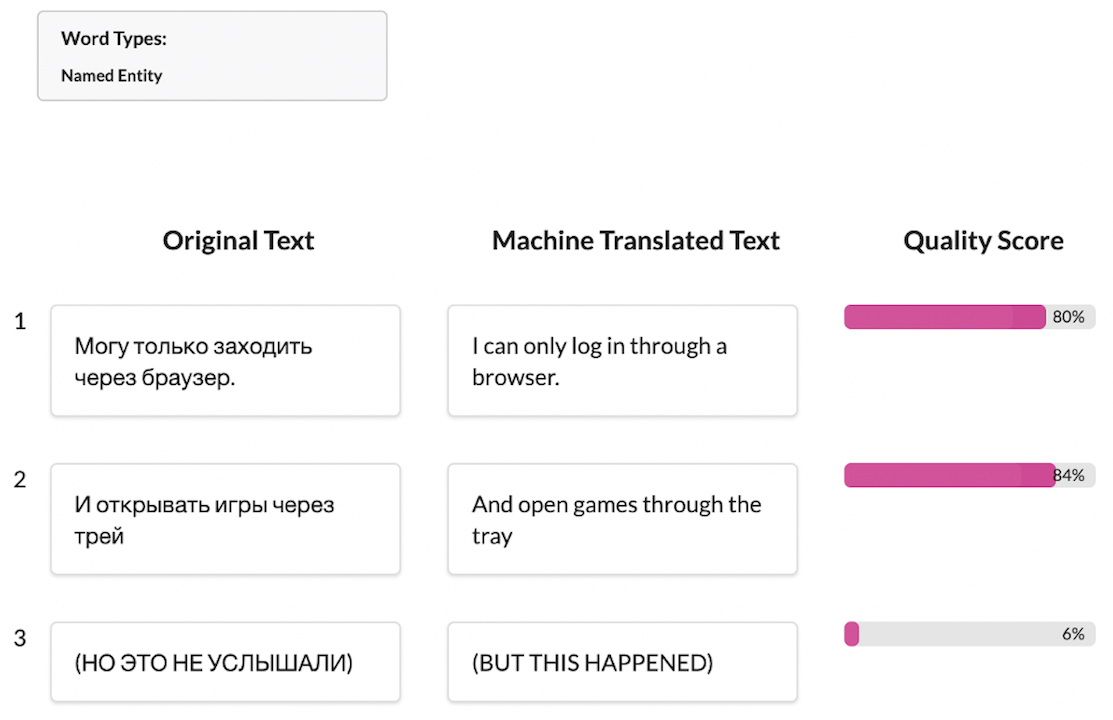
\includegraphics[width=\linewidth]{p1_v_0.png} 
        \caption{Passage 1 (passage type 1), Human Quality condition} \label{fig:p1_human_quality}
    \end{subfigure}
    \hfill
     \begin{subfigure}[t]{0.45\textwidth}
        \centering
        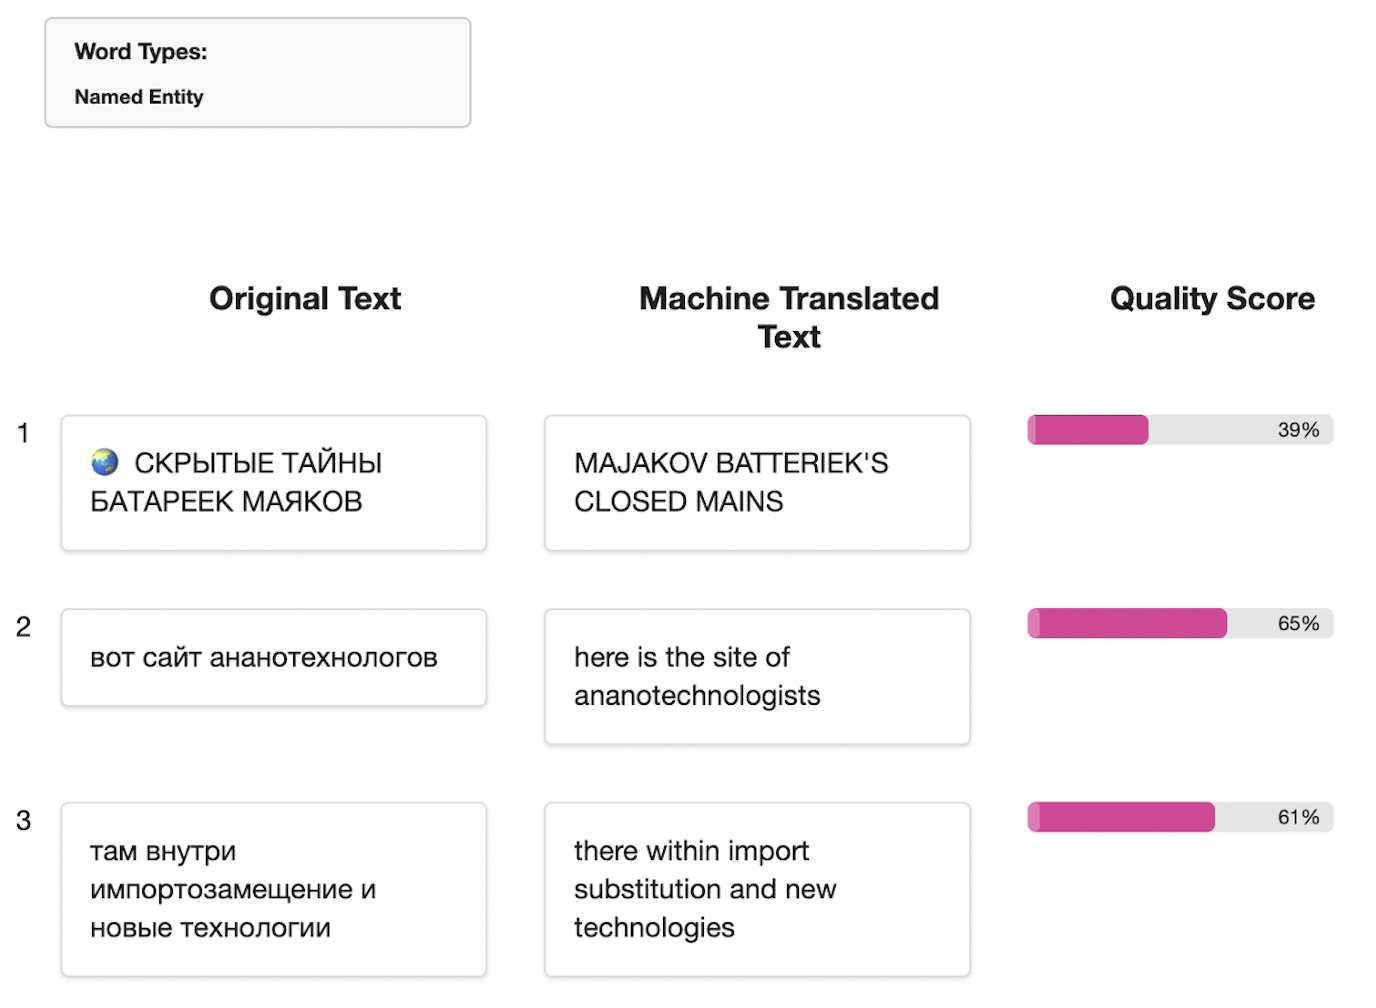
\includegraphics[width=\linewidth]{p3_p_0.png} 
        \caption{Passage 3 (passage type 2), Predicted Quality condition} \label{fig:p3_predicted_quality}
    \end{subfigure}
    
    \caption{Select examples of stimuli. All stimuli are available in supplemental materials.}
    \label{fig:exp_stim}
    
\end{figure}

\section{VeriCAT System Overview}
VeriCAT is designed to help analysts quickly and efficiently identify Russian $\rightarrow$ English MT sentences with poor translation quality, particularly in cases where fluency is a poor proxy for translation quality. %VeriCAT predicts quality scores for Russian $\rightarrow$ English translations generated by the pretrained FairSeq model~\cite{ott-etal-2019-fairseq} that performed best at WMT 2019 (news task, the most recent results from the annual benchmark for MT).
%VeriCAT is novel in that it uses QE as a means of communicating to the user whether a specific sentence of translated text is trustworthy. 
Commonly used MT accuracy metrics such as BLEU score~\cite{papineni-etal-2002-bleu} provide information about the accuracy of a MT model in general, (for example, FairSeq has a BLEU score of 40.0 on Russian to English translation, calculated with the SacreBLEU standard \cite{post-2018-call}) but, unlike VeriCAT, they do not provide feedback on individual translated sentences.  
%Our goal was to design a system that provides contextual information for \textit{individual snippets} of translated text, as opposed to the quality of the MT model as a whole.    
Below, we describe the training dataset for VeriCAT's QE model, the QE model itself, and VeriCAT's user interface.    

\subsection{Training Dataset}
The VeriCAT QE model is finetuned on a dataset composed of 7,000 labeled sentence pairs. The source of this text is passages from Reddit or Russian Proverbs from wikiquotes. The training dataset is curated from these sources because they represent types of text on which machine translation models are challenged. Each sentence is translated using the pretrained FairSeq model~\cite{ott-etal-2019-fairseq} that performed best at WMT 2019 (news task, the most recent results from the annual benchmark for MT). Each sentence has 3 Direct Assessment (DA) score quality judgments by human translators. These DA scores were labeled by ModelFront. Each DA score is rated on a scale from 1-100, with 100 representing a perfect translation. Across the dataset the average score is 68. These labeled data were also contributed to the World Machine Translation Workshop (Nov 2020) as part of the Quality Estimation Shared Task\footnote{statmt.org/wmt20}.  


\subsection{Quality Estimation Model}
Quality Estimation benchmarks are set annually at the World Machine Translation (WMT) QE Shared task. At the time of this study, the most accurate QE model available in the open source is the Predictor-Estimator model~\cite{Kim2017PredictorEstimatorUM}, open-sourced by OpenKiwi\footnote{https://github.com/Unbabel/OpenKiwi/tree/master/kiwi}~\cite{UnBabel} and the benchmark for WMT 2020. We pretrained the predictor model on the same parallel datasets the FairSeq translation model~\cite{ott-etal-2019-fairseq} was trained on. We finetuned the estimator model on the novel Russian-English QE dataset detailed above, tuning the following hyperparameters from the baseline model: epochs, hidden LSTM layers, learning rate, batch size, and dropout. We obtained a Pearson correlation of 0.62 on the development set, which we used to test since the shared task test set was not known to us. We ran inference with this model to generate the predictions for the VeriCAT UI, and confirmed the correlation between predicted and actual scores for this data subset was 0.67, in line with the model's expected performance. 


\subsection{User Interface}

The VeriCAT user interface is designed to provide context to help users assess the trustworthiness of a Russian $\rightarrow$ English translation via the FairSeq model.
Following Tufte's advice of \textit{above all else show the data}, the VeriCAT interface is designed simply, with a high data-ink ratio~\cite{tufte}.  
In the VeriCAT user interface, a passage of text is broken down into individual sentences. For each sentence, users see the original (Russian) text, the FairSeq translation (English), and VeriCAT’s quality score for that sentence (Figure \ref{fig:p3_predicted_quality}). Quality scores are represented with a simple horizontal bar, where the percentage of the bar that is colored represents the score on a scale from 1 to 100. For clarity, the numerical value of the quality score is also displayed. Unlike the uncertainty lattice developed by Collins et al.~\cite{collins2007lattices}, which drills down to word-level uncertainty, our approach focuses on sentences as a whole. These sentence-level quality scores are intended to help users quickly assess the translation quality for each sentence, to determine if it needs further inspection by a human. 


%\ab{I think we might want to move this next paragraph to future work instead of here. I'm just thinking since we don't test this version or provide a use case for it it might feel a little out of flow for new readers. Alternatively I think we could talk about this version first and say we came to the version we test through iterative design.}

%In addition to the version described above, we created a training version of VeriCAT.
%With this version, when viewing the training dataset, users have the option to switch to “God-mode” which allows them to see the hand-corrected version of each translated sentence — a “ground truth” for the dataset. In this mode, the interface also shows world-level errors in the translated text. Incorrect words are displayed in red, missing words are indicated with an underscore, and deletions are shown in red text with a strikethrough. Types of errors per sentence are aggregated and summarized below the Quality Score for each sentence. %An example of this version of VeriCAT is shown in Figure \ref{fig:teaser}.  


%https://github.com/Lab41/VeriCAT-UI

  



\section{Quantitative Evaluation: Machine vs. Human Quality Scores} 

In this experiment, we test whether the VeriCAT UI improves users' ability to identify translated text that is untrustworthy and should be re-translated by a human. We test the UI with ground truth DA quality scores generated by humans, and with VeriCAT QE scores. The following sections outline the study in more detail. 

%\subsection{Explanation Techniques}
\subsection{Sentence-level Quality Estimates}
%\ab{maybe rename to something like this?}

For this experiment we test a baseline version of the VeriCAT UI with no QEs (No XAI), a version in which ground truth DA QE' are shown (Human Quality), and a version in which VeriCAT QE (Predicted Quality) scores are shown (Figure \ref{fig:exp_stim}). This results in a 3 condition between-subjects experiment. 
%We include the Human Quality condition in an effort to isolate user performance issues due to ambiguous quality scores from performance issues due to quality scores in general. In other words, because the QE model scores are not perfect we included a ``perfect" version of quality scores to determine whether quality scores could improve user performance even in the best case. 
The Human Quality and Predicted Quality conditions are described in more detail below.  

\begin{compacthang}
    \item \textbf{Human Quality} DA quality scores are shown to users as percentages and progress bars, as shown in Figure \ref{fig:p1_human_quality}. We included only sentences with clearly good (> 70) or poor (< 30) quality scores to avoid the confounding factor of no clear difference between high and low quality scores. We include this condition, because VeriCAT QEs are not always sufficiently differentiated between high and low and we wanted to see if in the best case (i.e. with highly discriminate ground-truth scores) quality scores can improve user performance.  

    \item \textbf{Predicted Quality} VeriCAT QE scores are are shown to users as percentages and progress bars, as shown in Figure \ref{fig:p3_predicted_quality}.
    Unlike the ground truth DA scores used in the Human Quality condition, the QE scores are imperfect, and vary less between good and poor. Our goal in including predicted quality scores alongside ground truth scores is to understand if they perform significantly worse than best case quality scores. 
     %Or in other words, to see if QE modeling needs to be significantly improved before it can be useful for an application such as VeriCAT. Figure \ref{fig:p3_predicted_quality} shows an example of this condition. Notice that the magnitude of difference between high and low quality scores in the Human Quality condition is much larger than that in the  Predicted Quality condition (Figure \ref{fig:p1_human_quality} vs \ref{fig:p3_predicted_quality}).   
    
\end{compacthang}

\subsection{Passage Type}
We postulate that without XAI users will rely on fluency as a proxy for translation quality. Prior work shows that this is the case when it comes to trust of MT \cite{martindaleFluency2018}. However, there are cases where this technique fails as described in Section \ref{sec:design_requirements}.  
Each sentence in a passage can fall into one of four categories: (1) \textit{poor fluency + poor quality}, (2) \textit{poor fluency + good quality}, (3) \textit{good fluency + poor quality}, (4) \textit{good fluency + good quality}. Of these, we expect  sentences in the \textit{good fluency + poor quality}, and \textit{poor fluency + good quality} categories to be the most difficult for participants to assess. To test if these different sentence types have an effect on participants’ performance we arrange two different types of passages described below: 

\begin{compacthang}
    \item \textbf{Type 1} \textit{Good fluency + good quality, good fluency + poor quality, poor fluency + good quality}. Passage 1 is of this type and is shown in Figure \ref{fig:p1_human_quality}.    

    \item \textbf{Type 2} \textit{Good fluency + good quality, poor fluency + good quality, poor fluency + poor quality}. Passage 3 is of this type and is shown in Figure \ref{fig:p3_predicted_quality}.     
\end{compacthang}

Both of these passage types are designed to test if participants in an XAI condition will heed quality scores or their own intuition based on fluency to identify poor quality translations. 

\begin{figure}
    \centering
    
    \begin{subfigure}[t]{0.45\textwidth}
        \centering
        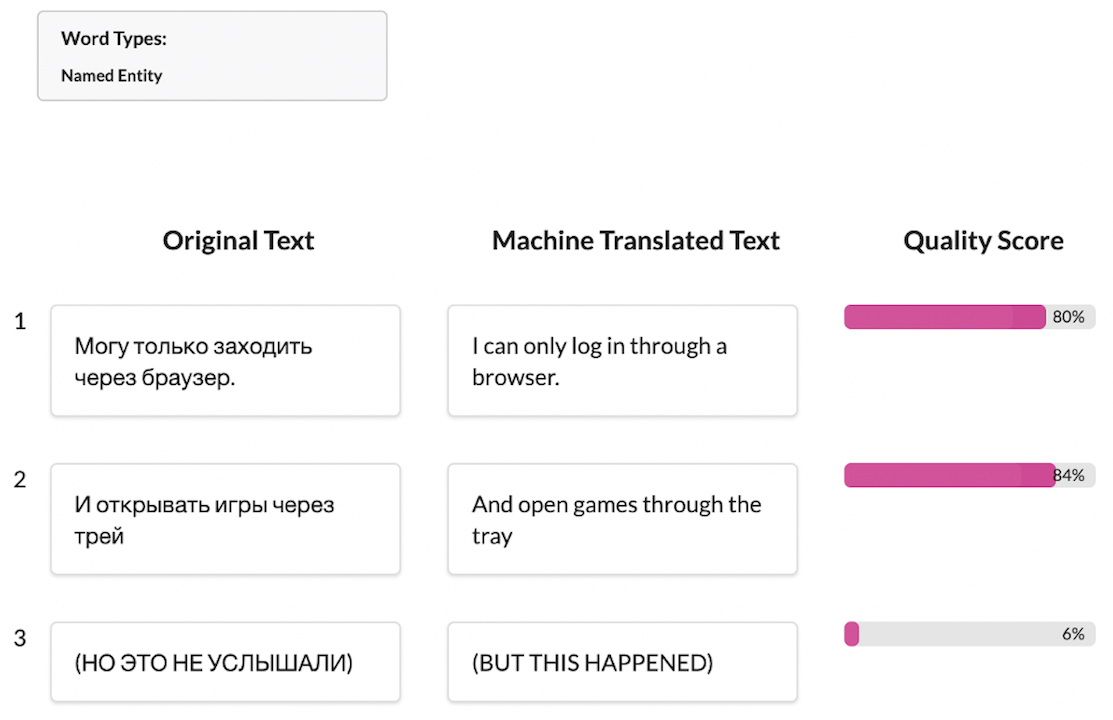
\includegraphics[width=\linewidth]{p1_v_0.png} 
        \caption{Passage 1 (passage type 1), Human Quality condition} \label{fig:p1_human_quality}
    \end{subfigure}
    \hfill
     \begin{subfigure}[t]{0.45\textwidth}
        \centering
        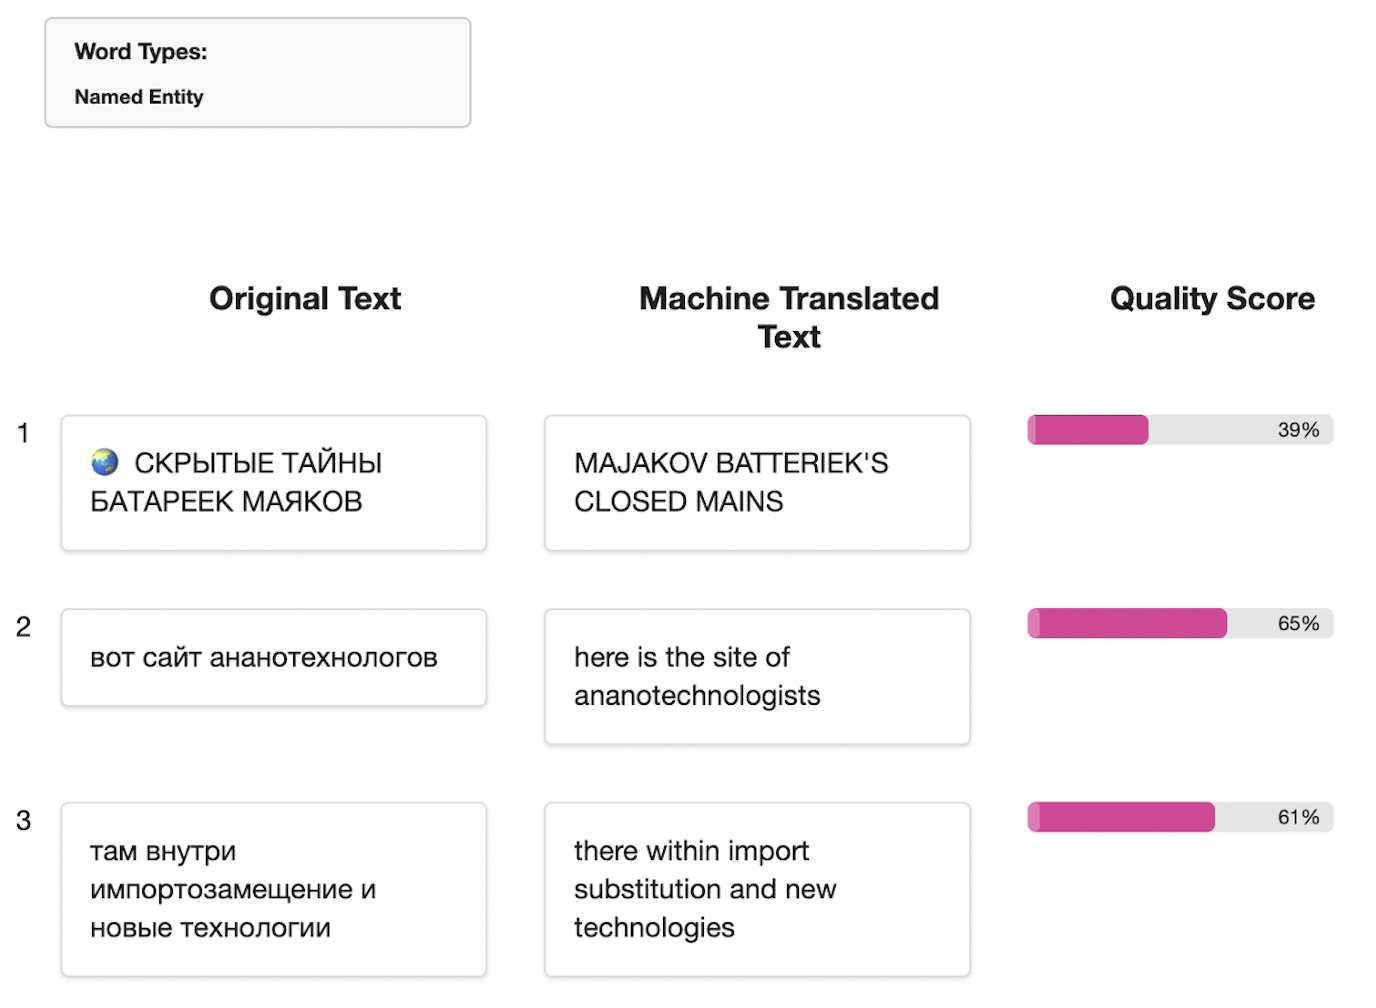
\includegraphics[width=\linewidth]{p3_p_0.png} 
        \caption{Passage 3 (passage type 2), Predicted Quality condition} \label{fig:p3_predicted_quality}
    \end{subfigure}
    
    \caption{Select examples of stimuli. All stimuli are available in supplemental materials.}
    \label{fig:exp_stim}
    
\end{figure}

\subsection{Task} 
We run a 3 condition experiment where each condition consists of a different XAI technique. Within each condition we include 2 passages of type 1 followed by 2 of type 2. The experimental task replicates an analyst determining if a MT needs a human translation as closely as possible within a controlled setting. For each passage the user is asked to look at the passage of text (comprised of 3 sentences), decide if any of the sentences in the passage should be re-translated by a human, and then answer 2 information retrieval questions based on the passage. The prompt before each passage is as follows:

\begin{quote}
Below is a passage written in Russian with an English translation generated by artificial intelligence. When you are ready, you will be asked to answer two comprehension questions. \textbf{You may select up to one section of the passage for re-translation by a human.} We recommend selecting the section you judge to have the poorest machine translation for re-translation by a human. 

Click ``I’m ready to see the questions'' when you are ready to see the comprehension questions. \textbf{If you would like a human re-translation of any section of the passage you must request it BEFORE you click ``I’m ready to see the questions''.} Once you click ``I’m ready to see the questions'', comprehension questions will appear on the page alongside the Russian test, English Machine translation, and any human translations you requested.  
\end{quote}

Participants were then given the chance to select sentence 1, 2, or 3 of the passage for re-translation by a human, or no-retranslation. After their selection, the original passage and machine translation remained on the screen in addition to the human translation of whichever sentence they selected for re-translation, and two information retrieval questions. 

\begin{table}[]
\resizebox{0.60\textwidth}{!}{%
\begin{tabular}{c|c|c}
\hline
\begin{tabular}[c]{@{}c@{}}Human Quality Score XAI\\ (Human Quality)\end{tabular} & \begin{tabular}[c]{@{}c@{}}Predicted Quality Score XAI\\ (Predicted Quality)\end{tabular} &  \begin{tabular}[c]{@{}c@{}}No XAI\\ (No XAI)\end{tabular} \\ \hline
                                                                    59                                                                       & 59                                                                                         & 47                                                        \\ \hline
\end{tabular}
}
\caption{N for each condition. }
\label{tab:exp_N}
\end{table}

\subsection{Participants} 

We recruited 193 participants from Amazon Mechanical Turk. Participation was restricted to
workers in the United States with an approval rating of greater than 90 percent. Participants were paid a base rate of USD $1.60$ for participation. Before analysis, participants who answered information retrieval questions for passage 1 and passage 2 (attention check questions) incorrectly were dropped from analysis ($N = 28$).  This left $N = 165$ participants distributed among stimuli as shown in Table \ref{tab:exp_N}. Demographics of participants are shown in Table \ref{tab:exp_demo}.


\begin{table}[h!]
\begin{threeparttable}[b]
\begin{tabular}{ll}
\hline
N                                                                                & 165                                                                                                                                                    \\ \hline
Age                                                                              & \begin{tabular}[c]{@{}l@{}}18-24: 6.7\%, 25-34: 45.5\%, 35-44: 24.8\%, \\ 45-54: 14.5\%, 55-64: 7.3\%, 65+: 1.2\%\end{tabular}                                     \\ \hline
Gender                                                                           & \begin{tabular}[c]{@{}l@{}}Female: 38.2\%, Male: 61.2\%, Non-binary: 0.6\%\end{tabular}                                                             \\ \hline
Education                                                                        & \begin{tabular}[c]{@{}l@{}}High School: 13.3\%, Associates: 12.1\%, Bachelors: 60.0\%, \\ Masters: 11.5\%, Professional: 2.4\%, Doctorate: 0.6\%\end{tabular}                            \\ \hline
\end{tabular}
\end{threeparttable}
\caption{Participant demographics.}
\label{tab:exp_demo}
\end{table}

\subsection{Procedure}

The experiment followed an approved protocol per redacted\_for\_anonymity’s company policy, and was posted as a HIT on Amazon Mechanical Turk. Workers who accepted the HIT followed a link to the experiment. After providing informed consent, participants were taken to an instruction page explaining the experiment. This page explained that they would see 4 passages of text translated from Russian to English by AI. They were told that they would be asked to answer two comprehension questions for each passage, but before doing so would have the opportunity to see one of the sentences in the passage re-translated by a human. After the instruction page, participants were shown the four passages one at a time. Participants could take as much time with each stimulus as they wanted before clicking a button to select which section of the passage they wanted re-translated and viewing the passage questions. After completing the main task, participants were asked to complete a short post-experiment questionnaire, the Tolerance for Ambiguity Survey from Geller et al. 1993 \cite{gellerTolerance1993}, a short demographic questionnaire, and to provide any additional feedback they wished.

\subsection{Hypotheses}

%We postulate that providing quality estimations for each sentence will help participants identify the sentence of lowest quality for re-translation only in cases where there is a significant difference between scores. In other words, we expect participants in the Human Quality condition to perform significantly better than participants in the Predicted Quality condition. 

To evaluate the VeriCAT system with Human vs Predicted Quality Scores, we test the following hypotheses:

\begin{compacthang}
    \item \textbf{H1}: Participants in the XAI conditions will have higher accuracy in identifying which sentence in a passage is of low quality and should be re-translated than participants with No XAI. 
    \item \textbf{H2}: Participants in the XAI conditions will have a greater change in trust of machine translation than participants in the No XAI condition. 
    \item \textbf{H3}: Participants’ tolerance for ambiguity will correlate with how well they are able to use the Predicted Quality XAI to perform the experimental task. 
    \item \textbf{H4}: Participants’ experience using machine translation will correlate with how well they are able to use XAI to perform the experimental task. 
    \item \textbf{H5}: Participants’ self-rated expertise in AI, MT, visualization, and statistics will correlate with how well they are able to use XAI to perform the experimental task.   
\end{compacthang}

\subsection{Findings}

We consider a participant’s answer correct if they select the sentence in a passage with the lowest quality score as the one to get re-translated by a human. To calculate overall accuracy, we sum the number of correct answers across all four passages and divide by 4. The following analyses use this outcome measure to test the hypotheses listed above.

\subsubsection{Does XAI help?}

We start by looking at which sentences people chose to re-translate for each condition and passage. For all passages, we see participants in both Quality conditions are on average most accurate at selecting the correct sentence for re-translation. Interestingly, we see that participants in the No XAI condition often opt for no-retranslation. Proportions of participants giving each answer for each passage and condition are shown in Figure \ref{fig:exp_prop_answers}.

\begin{figure}*
    \centering
    
    \cbox{bar-noXai} \textit{No XAI} \quad
    \cbox{bar-Qual} \textit{Human Quality} \quad
    \cbox{bar-PredictQ} \textit{Predicted Quality} \quad
    
    \begin{subfigure}[t]{0.45\textwidth}
        \centering
        \scalebox{0.7}{
        \begin{bchart}[step=.25,max=1,width=\linewidth]
        \bcbar[color=bar-noXai]{.06}
        \bclabel{\textit{Good Fluency}}
        \bcbar[color=bar-Qual]{.51}
        \bclabel{\textit{Poor score}}
        \bcbar[color=bar-PredictQ]{.37}
        \bcskip{6pt}
        
        \bcbar[color=bar-noXai]{.15}
        \bclabel{\textit{Good Fluency}}
        \bcbar[color=bar-Qual]{.15}
        \bclabel{\textit{Good score}}
        \bcbar[color=bar-PredictQ]{.07}
        \bcskip{6pt}
        
        \bcbar[color=bar-noXai]{.38}
        \bclabel{\textit{Poor Fluency}}
        \bcbar[color=bar-Qual]{.14}
        \bclabel{\textit{Good score}}
        \bcbar[color=bar-PredictQ]{.31}
        \bcskip{6pt}
        
        \bcbar[color=bar-noXai]{.40}
        \bclabel{\textit{No}}
        \bcbar[color=bar-Qual]{.20}
        \bclabel{\textit{Re-translation}}
        \bcbar[color=bar-PredictQ]{.25}
        
        \bcxlabel{Proportion of Participants Selecting}
        \end{bchart}}
        \caption{Passage 1} 
        \label{fig:exp_p1_prop_answers}
    \end{subfigure}
    \hfill
    \begin{subfigure}[t]{0.45\textwidth}
        \centering
        \scalebox{0.7}{
        \begin{bchart}[step=.25,max=1,width=\linewidth]
        \bcbar[color=bar-noXai]{.06}
        \bclabel{\textit{Good Fluency}}
        \bcbar[color=bar-Qual]{.53}
        \bclabel{\textit{Poor score}}
        \bcbar[color=bar-PredictQ]{.37}
        \bcskip{6pt}
        
        \bcbar[color=bar-noXai]{.13}
        \bclabel{\textit{Good Fluency}}
        \bcbar[color=bar-Qual]{.12}
        \bclabel{\textit{Good score}}
        \bcbar[color=bar-PredictQ]{.08}
        \bcskip{6pt}
        
        \bcbar[color=bar-noXai]{.21}
        \bclabel{\textit{Poor Fluency}}
        \bcbar[color=bar-Qual]{.15}
        \bclabel{\textit{Good score}}
        \bcbar[color=bar-PredictQ]{.20}
        \bcskip{6pt}
        
        \bcbar[color=bar-noXai]{.60}
        \bclabel{\textit{No}}
        \bcbar[color=bar-Qual]{.20}
        \bclabel{\textit{Re-translation}}
        \bcbar[color=bar-PredictQ]{.34}
        
        \bcxlabel{Proportion of Participants Selecting}
        \end{bchart}}
        \caption{Passage 2} 
        \label{fig:exp_p2_prop_answers}
    \end{subfigure}
    \hfill
     \begin{subfigure}[t]{0.45\textwidth}
        \centering
        \scalebox{0.7}{
        \begin{bchart}[step=.25,max=1,width=\linewidth]
        \bcbar[color=bar-noXai]{.26}
        \bclabel{\textit{Poor Fluency}}
        \bcbar[color=bar-Qual]{.69}
        \bclabel{\textit{Poor score}}
        \bcbar[color=bar-PredictQ]{.68}
        \bcskip{6pt}
        
        \bcbar[color=bar-noXai]{.19}
        \bclabel{\textit{Poor Fluency}}
        \bcbar[color=bar-Qual]{.05}
        \bclabel{\textit{Good score}}
        \bcbar[color=bar-PredictQ]{.15}
        \bcskip{6pt}
        
        \bcbar[color=bar-noXai]{.09}
        \bclabel{\textit{Good Fluency}}
        \bcbar[color=bar-Qual]{.10}
        \bclabel{\textit{Good score}}
        \bcbar[color=bar-PredictQ]{.03}
        \bcskip{6pt}
        
        \bcbar[color=bar-noXai]{.47}
        \bclabel{\textit{No}}
        \bcbar[color=bar-Qual]{.15}
        \bclabel{\textit{Re-translation}}
        \bcbar[color=bar-PredictQ]{.14}
        
        \bcxlabel{Proportion of Participants Selecting}
        \end{bchart}}
        \caption{Passage 3} 
        \label{fig:exp_p3_prop_answers}
    \end{subfigure}
    \hfill
    \begin{subfigure}[t]{0.45\textwidth}
        \centering
        \scalebox{0.7}{
        \begin{bchart}[step=.25,max=1,width=\linewidth]
        \bcbar[color=bar-noXai]{.45}
        \bclabel{\textit{Poor Fluency}}
        \bcbar[color=bar-Qual]{.64}
        \bclabel{\textit{Poor score}}
        \bcbar[color=bar-PredictQ]{.64}
        \bcskip{6pt}
        
        \bcbar[color=bar-noXai]{.02}
        \bclabel{\textit{Poor Fluency}}
        \bcbar[color=bar-Qual]{.12}
        \bclabel{\textit{Good score}}
        \bcbar[color=bar-PredictQ]{.08}
        \bcskip{6pt}
        
        \bcbar[color=bar-noXai]{.11}
        \bclabel{\textit{Good Fluency}}
        \bcbar[color=bar-Qual]{.10}
        \bclabel{\textit{Good score}}
        \bcbar[color=bar-PredictQ]{.12}
        \bcskip{6pt}
        
        \bcbar[color=bar-noXai]{.43}
        \bclabel{\textit{No}}
        \bcbar[color=bar-Qual]{.14}
        \bclabel{\textit{Re-translation}}
        \bcbar[color=bar-PredictQ]{.15}
        
        \bcxlabel{Proportion of Participants Selecting}
        \end{bchart}}
        \caption{Passage 4} 
        \label{fig:exp_p4_prop_answers}
    \end{subfigure}
    
    \caption{Proportions of participants selecting each type of sentence for re-translation by passage.}
    \label{fig:exp_prop_answers}

\end{figure}

To test if the differences we observe are significant we ran a Kruskal-Wallis test of $overall\_score \sim condition$ \footnote{We use a Kruskal-Wallis test because according to the Shapiro-Wilk Normality test $overall\_score$ is not normally distributed ($W = 0.87, p < 0.001$).} and find a significant difference across conditions ($H(2) = 29.7, p < 0.001$). A post-hoc Dunn’s multiple comparisons test with a Bonferroni corrected alpha ($0.02$) shows significant pairwise differences between Human Quality and No XAI ($Z = 5.2, p < 0.01$), and No XAI and Predicted Quality ($Z = -4.3, p < 0.01$). Figure \ref{fig:exp_overall_distribution} shows $overall\_score$ distributions by condition. 

\begin{figure}[h!]
    \centering
    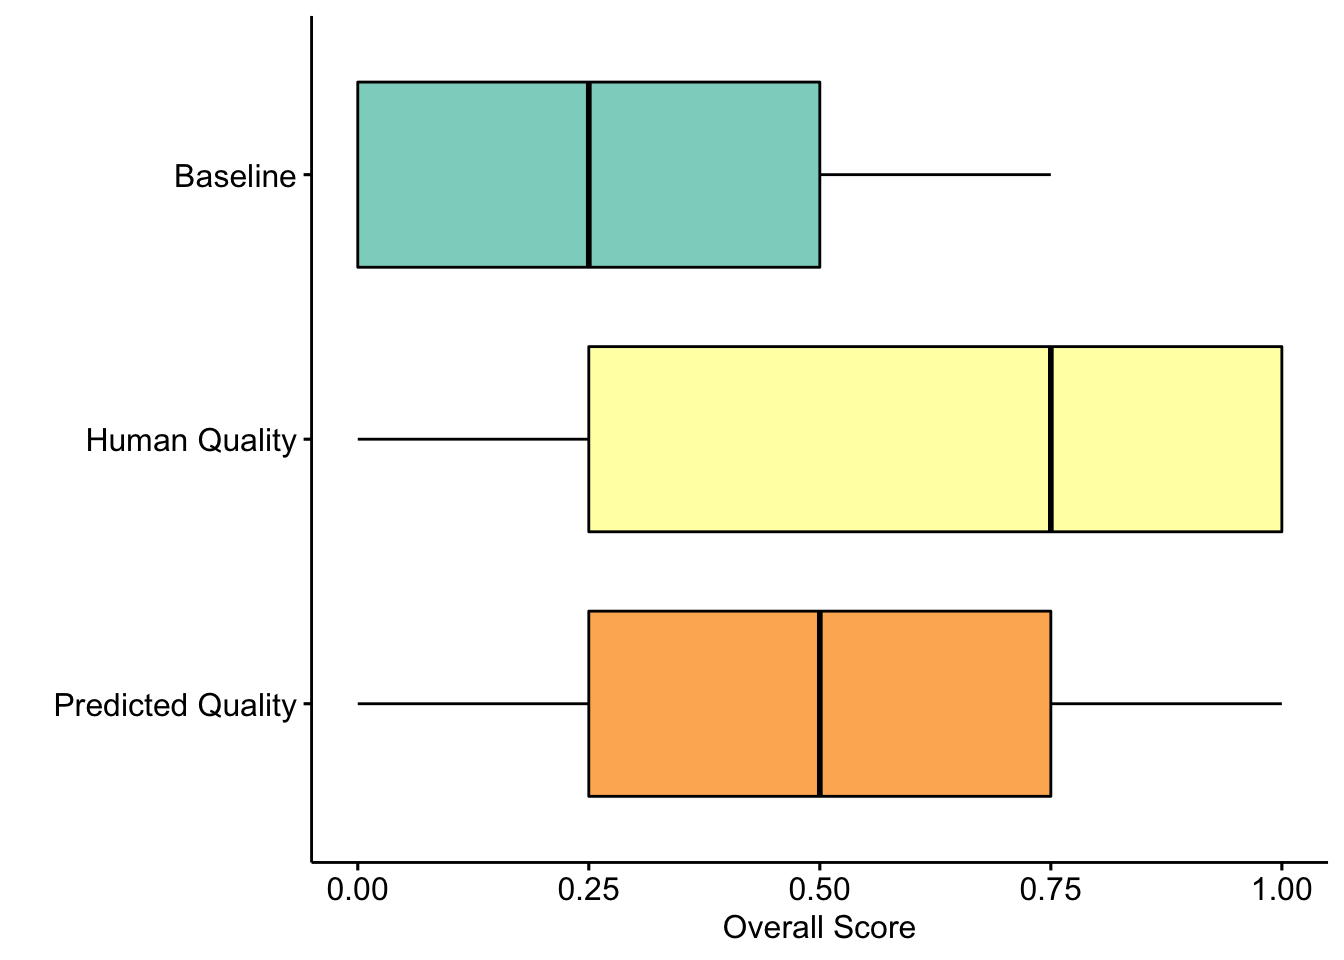
\includegraphics[width=0.50\textwidth]{exp2_overall_distribution.png}
    \caption{Boxplot of overall score by condition.}
    \label{fig:exp_overall_distribution}
\end{figure}

These results suggest that sentence-level quality scores can significantly improve participants’ performance over No XAI, regardless of if they are ground-truth or model predictions. Therefore, we \textbf{accept H1}. The results also show that there is no significant difference in performance between ground-truth and predicted quality scores, suggesting that though imperfect, predicted quality scores are as effective as DA quality scores. 

\subsubsection{Does XAI affect trust?}

We asked participants before the experimental task “Please rate how much you trust artificial intelligence to correctly translate sentences from a language you do not speak into a language you do speak from 1 (No trust) to 5 (Complete trust).”  We asked the same question at the end of the experiment. To analyze whether different conditions changed participants' trust in machine translation, we calculated $delta\_trust$ for each participant by subtracting their answer to the pre-experimental task trust question from their answer to the post-experimental task trust question. 

We run a Kruskal-Wallis test of $delta\_trust \sim condition$ \footnote{We use a Kruskal-Wallis test because according to the Shapiro-Wilk Normality test $delta\_trust$ is not normally distributed ($W = 0.74, p < 0.001$).} and find no significant difference across conditions ($H(2) = 3.5, p = 0.17$). This suggests that neither the presence of XAI nor the different types of quality scores significantly affected participants’ trust in machine translation, thus we \textbf{reject H2}. Average change in trust by condition is shown in Figure \ref{fig:exp_delta_trust}.

\begin{figure}[h!]
    \centering
    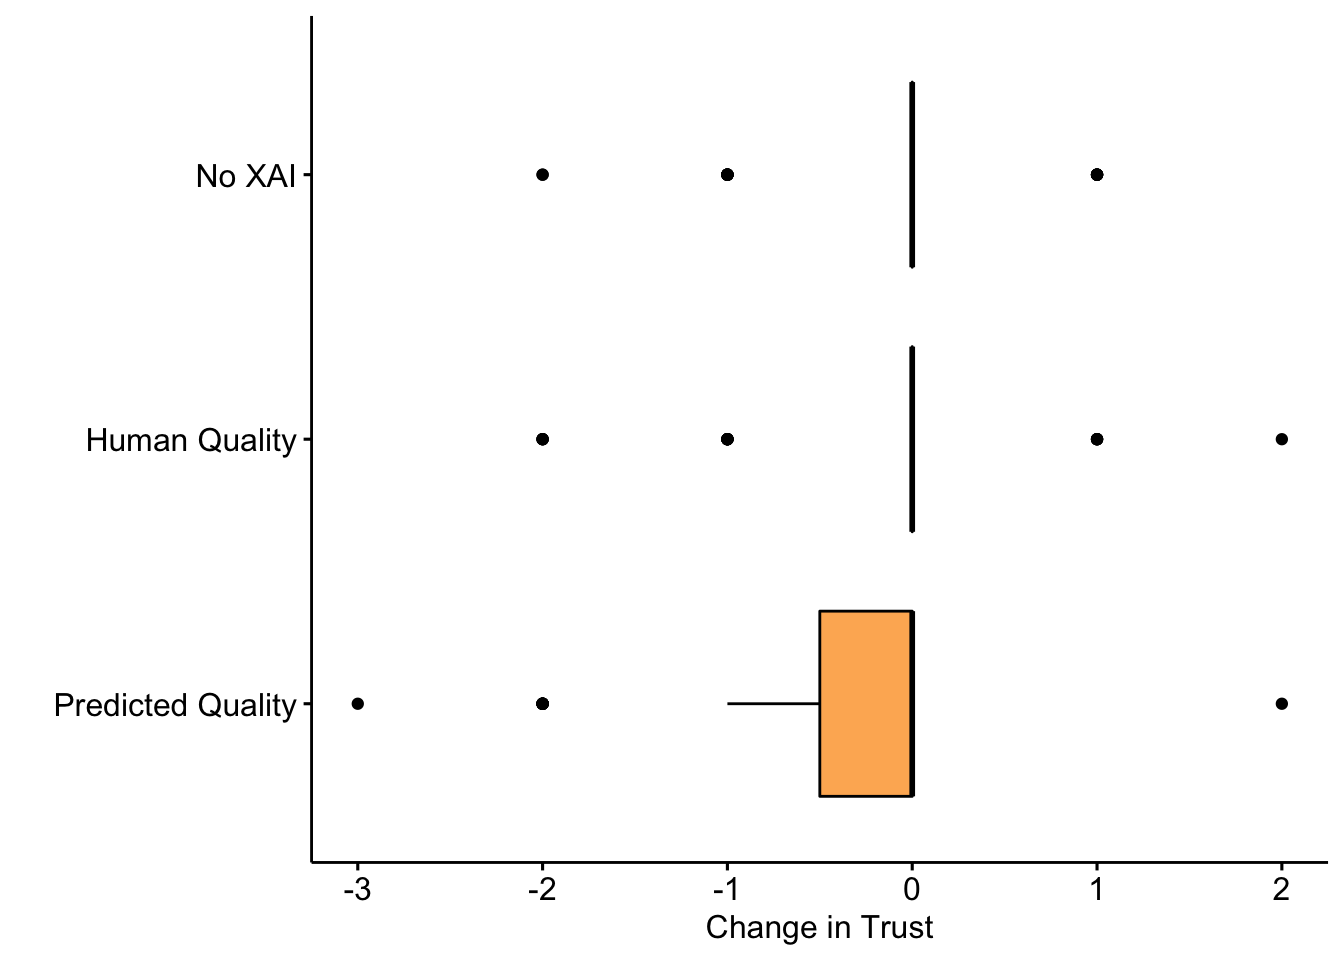
\includegraphics[width=0.50\textwidth]{exp2_delta_trust.png}
    \caption{Boxplot of change in trust by condition.}
    \label{fig:exp_delta_trust}
\end{figure}

\subsubsection{Is the efficacy of XAI influenced by participants' individual differences?}

Prior work has shown that individual user differences can play a strong role in how well users utilize a visualization for a problem solving task\cite{liuSurvey2020}. However, there has been little research investigating how individual differences can affect understanding, trust, and use of AI. In an effort to start answering this question we captured three different individual differences of users (intolerance for ambiguity, usage of MT, and self-rated expertise) and analysed whether there were any correlations between these measures and users’ $overall\_score$. Our findings follow.

\paragraph{Intolerance for Ambiguity} 

Given the survey instrument we use to measure Intolerance for Ambiguity\cite{gellerTolerance1993} participants’ scores could range from 7 (extremely low intolerance for ambiguity) to 49 (extremely high intolerance for ambiguity). The median score for intolerance for ambiguity of participants is 30. 

Within each condition we tested for a significant Pearson correlation between participants’ $overall\_score$ and $intolerance\_for\_ambiguity$. Regression lines for each condition are shown in Figure \ref{fig:exp_intol_ambiguity}. We find no significant correlation in any condition (Human Quality -- ($r(57) = -0.14, p = 0.29$), Predicted Quality --  ($r(57) = 0.03, p = 0.81$), No XAI -- ($r(45) = -0.01, p = 0.95)$). This suggests that intolerance for ambiguity has no effect on participants' performance, thus we \textbf{reject H3}. 

\begin{figure}[h!]
    \centering
    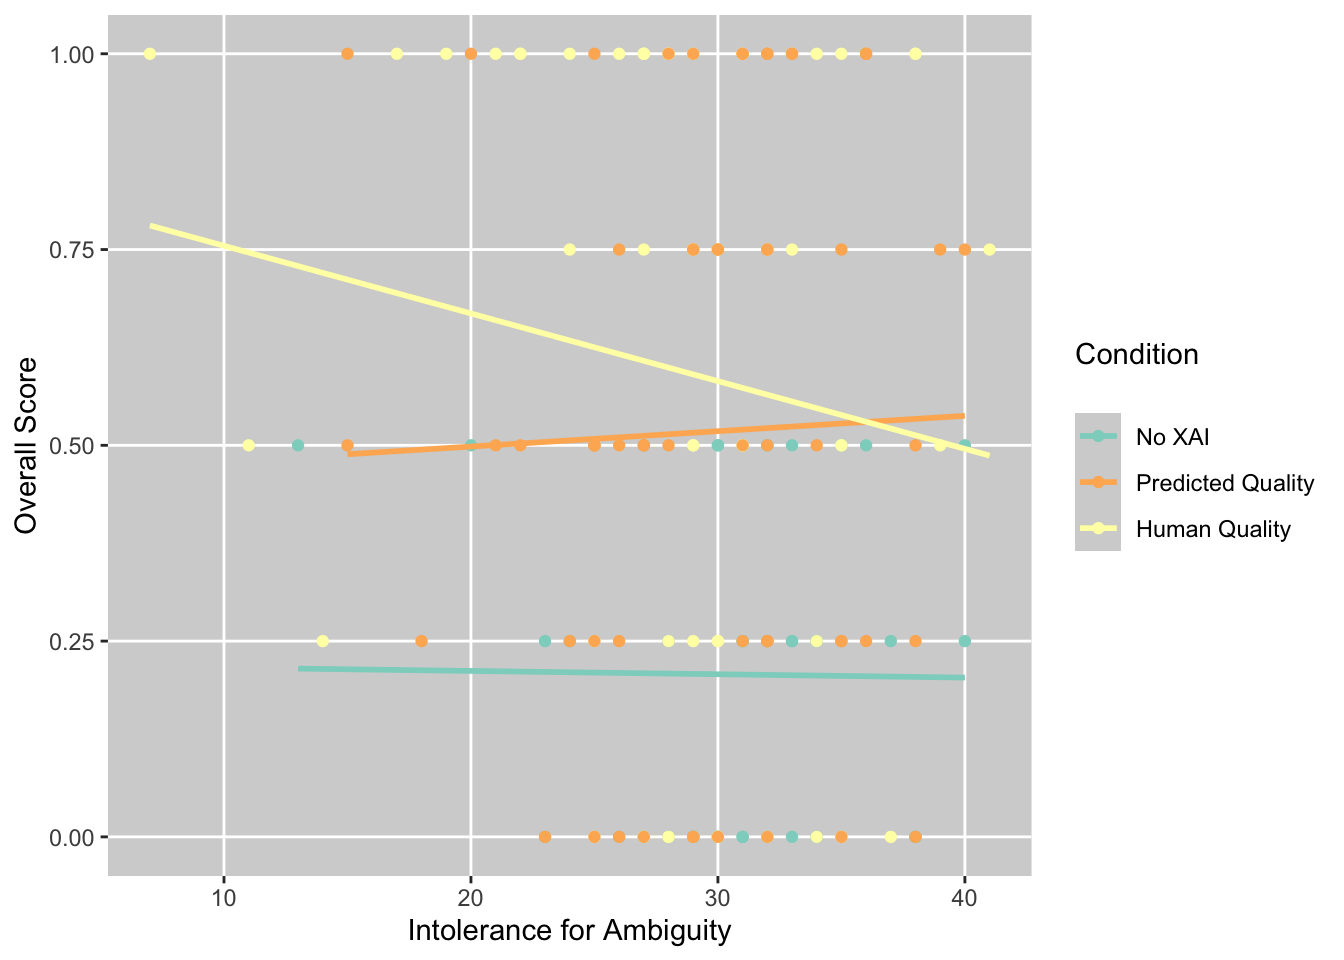
\includegraphics[width=0.50\textwidth]{exp2_intol_ambiguity.png}
    \caption{Regression lines of overall score and intolerance for ambiguity by condition.}
    \label{fig:exp_intol_ambiguity}
\end{figure}

\paragraph{Usage of Machine Translation} 

We ask participants to rank how often they use Google Translate and Facebook Translate on a five-point scale of Never, Yearly, Monthly, Weekly, Daily. We assign weights to each point in the scale ranging from 1 (Never) to 5 (Daily) and use these to calculate a machine translation usage score for each participant. The higher this score, the more often a participant indicated using MT. 

Within each condition we test for a Pearson correlation between participants’ frequency of MT usage and performance. Regression lines for each condition are shown in Figure \ref{fig:exp_MT_use}. We find a significant correlation between frequency of MT usage and overall score for participants in the Human Quality condition ($r(57) = -0.32, p < 0.05$), and no significant correlation in any other condition (Predicted Quality -- ($r(57) = -0.21, p = 0.11$), No XAI -- ($r(45) = -0.23, p = 0.11$)). This suggests that in the Human Quality condition as participants’ frequency of MT usage increases, their performance decreases, thus we \textbf{partially accept H4}.

\begin{figure}[h!]
    \centering
    \includegraphics[width=0.50\textwidth]{exp2_MT_use.png}
    \caption{Regression lines of overall score and frequency of MT usage by condition.}
    \label{fig:exp_MT_use}
\end{figure}

\paragraph{Self-rated Expertise}

We ask participants to rate their own expertise from 1 (Novice) to 5 (Expert) in four areas related to XAI: AI, MT, visualization, and statistics. We use these self ratings to test for correlations between participants’ self-rated expertise and performance. Regression lines for each condition are shown in Figure \ref{fig:exp_expert}.  

\begin{figure}[h!]
    \centering
    
    \cbox{bar-noXai} \textit{No XAI} \quad
    \cbox{bar-Qual} \textit{Human Quality} \quad
    \cbox{bar-PredictQ} \textit{Predicted Quality} \quad
    
    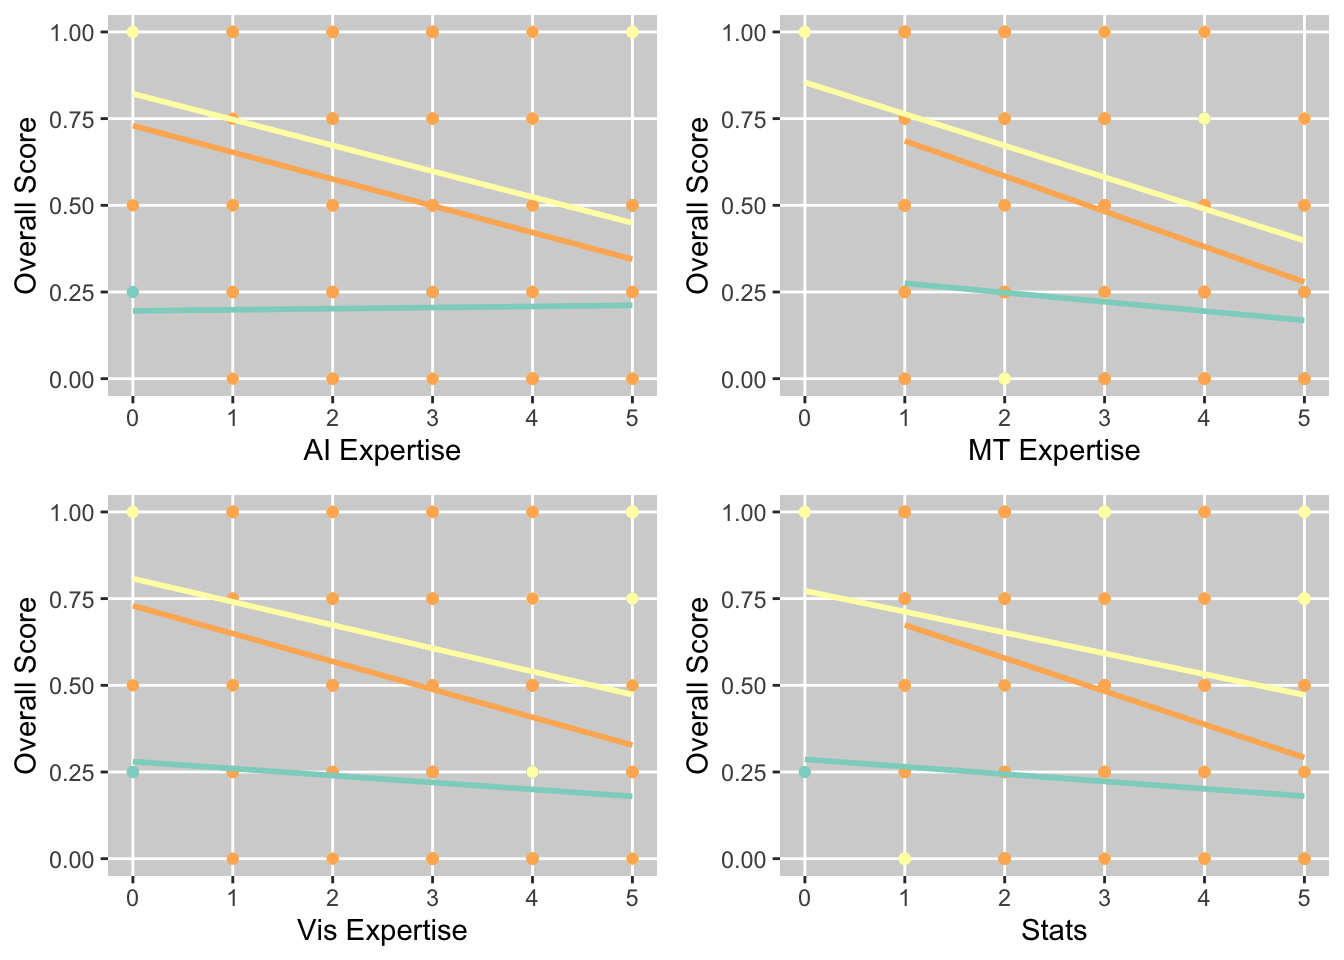
\includegraphics[width=0.50\textwidth]{exp2_expert.png}
    \caption{Regression lines of overall score and self-rated expertise by condition.}
    \label{fig:exp_expert}
\end{figure}

Within each condition we test for a Pearson correlation between each self-rated expertise and overall score. In the Human Quality, and Predicted Quality conditions we find a significant correlations between self rated expertise in AI and MT and $overall\_score$. In addition, we find significant correlations between self-rated expertise in visualization and statistics and overall score in the Predicted Quality condition.  
(Analysis results for all of these tests are listed in Table \ref{tab:exp1_expertise_stats}.) Overall, our results suggest that in all cases except for No XAI as self-rated expertise in AI and MT (and in the case of Predicted Quality visualization and statistics) increase, $overall\_score$ decreases, thus we \textbf{accept H5}.

\begin{table}[]
\resizebox{0.70\textwidth}{!}{%
\begin{tabular}{llc}
\hline
\multicolumn{1}{c}{Measure}                            & \multicolumn{1}{c}{Condition} & Result                                   \\ \hline
\multirow{4}{*}{Self-rated expertise in AI}            & Human Quality              & \textbf{r(57) = -0.27, p \textless 0.05} \\
                                                       & Predicted Quality          & \textbf{r(57) = -0.29, p \textless 0.05}         \\
                                                       & No XAI                     & r(45) = 0.02, p = 0.91                   \\ \hline
\multirow{4}{*}{Self-rated expertise in MT}            & Human Quality              & \textbf{r(57) = -0.31, p \textless 0.05} \\
                                                       & Predicted Quality          & \textbf{r(57) = -0.40, p \textless 0.01}          \\
                                                       & No XAI                     & r(45) = -0.13, p = 0.39                  \\ \hline
\multirow{4}{*}{Self-rated expertise in visualization} & Human Quality              & r(57) = -0.24, p = 0.06                  \\
                                                       & Predicted Quality          & \textbf{r(57) = -0.31, p \textless 0.05}                  \\
                                                       & No XAI                     & r(45) = -0.11, p = 0.48                  \\ \hline
\multirow{4}{*}{Self-rated expertise in statistics}    & Human Quality              & r(57) = -0.21, p = 0.10                  \\
                                                       & Predicted Quality          & \textbf{r(57) = -0.36, p \textless 0.01}          \\
                                                       & No XAI                     & r(45) = -0.11, p = 0.46                  \\ \hline
\end{tabular}%
}
\caption{Pearson correlation results for each self-rated expertise measure by condition. Significant results are in \textbf{bold}.}
\label{tab:exp1_expertise_stats}
\end{table}

\subsubsection{Qualitative Feedback}

Qualitative feedback from our study indicated that overall users were satisfied with the UI. A random sampling of participants were asked if they would have liked to see any additional information in the UI, and only 5 of the 66 participants asked this question said yes. Overall, we gathered very positive feedback from study participants. Many commented that it was a ``good" and ``interesting" study, and one participant (who was assigned to a quality score condition) went as far to say ``the task was enjoyable". This feedback indicates that the VeriCAT UI performs its intended purpose well, and does so without many (if any) negative effects on the user.       

\subsection{Discussion of Findings} 

The purpose this experiment was to test if showing users of MT text sentence-level quality scores of translations could improve performance in identifying poor quality machine translations. we find that both QE and ground-truth DA scores significantly improve user performance compared to No XAI. 
In addition, we find that although user performance is slightly lower with machine-generated quality scores, there is no significant difference in performance compared to human-generated quality scores. 

Unexpectedly, we find providing quality scores has no effect on participants' trust of MT. There are a few potential explanations for this. One is that participants in general come into the experiment with an appropriate amount of trust in MT quality. In this case, showing participants quality estimation for MT would help them perform the experimental task more accurately, but would not necessarily reveal to them that MT is less (or more) accurate than they already expected it to be. 

Another explanation could be that our experimental task is not realistic enough to force users to consider their trust of MT output. Future work should explore a similar study in which the experimental task comes at more of a stake to the user. For example, asking the user to flag sentences as inappropriate based on MT, or asking the user whether or not they would repost a passage based on the MT. Scenarios such as these may elicit a stronger evaluation of trust from participants.

Unlike participants in the Human Quality condition, we find no significant correlation between participants' overall score and frequency of MT use in the Predicted Quality condition. Similar to the Human Quality condition, we find a significant negative correlation between participants' self-rated expertise and overall score in the Predicted Quality condition.  

This finding is surprising, as we would expect people who are more familiar with MT through frequent usage to have a better understanding of its limitations and similarly we would expect people with more expertise in MT and AI to have a good understanding of MT limitations and of how to read and process quality indicators. We postulate that in both of these cases what we are observing is overconfidence leading to errors. We suspect that the more often one uses MT, the more the more familiar and comfortable they become with it and therefore see no need to rely on quality scores instead of themselves to identify poor translations. We suspect that the same is true of self-rated experts in MT and AI, and the better someone thinks they are at understanding the underlying mechanisms of MT the more likely they are to want to rely on their own quality assessments instead of those shown by XAI.

Our findings suggest that novices are likely to follow XAI guidance, while those with more familiarity or expertise in the area are likely to ignore XAI guidance in favor of their own judgement. This means that in designing XAI interfaces, designers should pay specific attention to this population and center their design around the unique needs of these users instead of complete novices. 

Finally our findings suggest that although the QE model is not perfect it currently performs well enough to be used as a part of MT XAI, and doing so will not introduce any additional burdens to different types of users. In fact, utilizing QE scores instead of DA scores may remove the potentially negative effect of prior MT usage on performance.  



\section{Qualitative Evaluation}
\section{Lessons Learned}

Through the process of conceptualizing, testing, and refining VeriCAT we show that MT output can be thought of as an XAI problem, and QE can be used to provide context to translations to guide users towards more appropriate trust of output. Below, we present several lessons learned from the evaluation of VeriCAT.     

\paragraph{\textbf{Test idealized explanations}} In Experiment 1 we test idealized versions of two explanation techniques for MT (word-level predicted errors and sentence-level quality estimations). While models exist for each technique, neither are perfect. One of our goals with Experiment 1 was to determine if either of these particular explanation techniques were useful enough to users to be worth further developing. 

We used this ``idealized" method to determine a goal post for each explanation technique. The thought behind this is that if the perfect hand crafted versions of either technique did not significantly improve participants' performance then that would be a clear indication that the technique was not worth further refinement. This happened with the word-level predicted error; which we found did not significantly improve participants' performance over No XAI. Thanks to this outcome we were able to refine our second experiment and remove the word-level predicted error condition from it. This saved time, effort, and money in the iterative development of VeriCAT.   

\paragraph{\textbf{Test for behaviors and beliefs}} According to prior work, one of the things people are asking for when they ask for XAI is an indication of whether they should trust a model or model output\cite{brennen2020What}. In this study we saw that adding XAI to MT did not significantly change participants' self-reported trust of MT. However, we did see a significant change in behavior when participants were exposed to XAI. In our experiments we observed that participants tend to opt for no re-translation when presented with a passage of machine translated text and no additional information. This suggests that participants may be over-trusting of the MT output, and see no reason to question any of the translations they see. In contrast, we observe participants in effective XAI conditions tend to opt for a human re-translation. This suggests a more appropriate level of trust in the MT output, as participants are choosing to double check portions of it. Based on this mismatch of self-reported trust and behavior, we recommend testing for changes in behavior as well as collecting self-reported measures as part of the the user-centered XAI process.    

\paragraph{\textbf{Plan for overconfidence}} Interestingly, we found negative correlations between participants' usage of MT tools and overall scores and between participants' self-rated expertise and overall scores. While we are well aware that correlation does not necessarily imply causation, we do strongly urge XAI designers to take this finding into consideration when designing tools. Our results imply that it may be necessary to make indications of poor translation quality more alarming to users who use MT more often. Similarly, users who have high confidence in their AI and MT expertise may need intensified warnings of poor translation quality compared to users with low confidence in these areas. In short, our results suggest that there is likely not a ``one size fits all" solution to XAI problem; in addition to customizing XAI design on a macro-level for various domains it should be customized on a micro-level to account for differences in individual users.   

\paragraph{\textbf{Employ a user-centered design process}} Perhaps the most important lesson learned in building and evaluating VeriCAT is that a user-centered design process is critical to XAI development. \ab{add more later}  

%Revisions to interface (\textbf{interface version 2})

%Insights about model design (\textbf{model version 3})

\section{Conclusion}



%%\input{sections/design_goals}
%%\input{sections/design_process}
%%
%% The acknowledgments section is defined using the "acks" environment
%% (and NOT an unnumbered section). This ensures the proper
%% identification of the section in the article metadata, and the
%% consistent spelling of the heading.
\begin{acks}
TBD
\end{acks}

%%
%% The next two lines define the bibliography style to be used, and
%% the bibliography file.
\bibliographystyle{ACM-Reference-Format}
\bibliography{main}


\end{document}
\endinput
%%
%% End of file `sample-authordraft.tex'.
